\documentclass{beamer}
\usepackage[utf8]{inputenc}
\usepackage{graphicx, epsfig}
\usepackage{amsmath,mathrsfs,amsfonts,amssymb}
%\usepackage{subfig}
\usepackage{floatflt}
\usepackage{epic,ecltree}
\usepackage{mathtext}
\usepackage{fancybox}
\usepackage{fancyhdr}
\usepackage{multirow}
\usepackage{enumerate}
\usepackage{epstopdf}
\usepackage{multicol}
\usepackage{algorithm}
\usepackage[noend]{algorithmic}
\def\algorithmicrequire{\textbf{Input:}}
\def\algorithmicensure{\textbf{Output:}}
\usetheme{default}%{Singapore}%{Warsaw}%{Warsaw}%{Darmstadt}
\usecolortheme{default}
\setbeamerfont{title}{size=\Huge}
\setbeamertemplate{footline}[page number]{}
\setbeamerfont{title}{size=\Huge}
\beamertemplatenavigationsymbolsempty

\newcommand{\bx}{\mathbf{x}} 
\newcommand{\bz}{\mathbf{z}} 
\newcommand{\by}{\mathbf{y}} 

\newcommand{\bX}{\mathbf{X}} 
\newcommand{\bZ}{\mathbf{Z}} 

\newcommand{\btheta}{\boldsymbol{\theta}} 
\newcommand{\bphi}{\boldsymbol{\phi}} 

\DeclareMathOperator*{\argmin}{arg\,min}
\DeclareMathOperator*{\argmax}{arg\,max}

%\definecolor{beamer@blendedblue}{RGB}{15,120,80}
%----------------------------------------------------------------------------------------------------------
\title[\hbox to 56mm{Deep Generative Models  \hfill\insertframenumber\,/\,\inserttotalframenumber}]
{Deep Generative Models \\ Lecture 1}
\author[Roman Isachenko]{\\Roman Isachenko}
\institute[Ozon]{Ozon Masters \\
}
\date{2021}
%--------------------------------------------------------------------------------
\begin{document}
%--------------------------------------------------------------------------------
\begin{frame}
%\thispagestyle{empty}
\titlepage
\end{frame}
%--------------------------------------------------------------------------------
\section{Logistics}
%=======
\begin{frame}{Logistics}
    \begin{itemize}
        \item homeworks: 30 points
        \begin{itemize}
            \item hw1: autoregressive models
            \item hw2: latent variable models
            \item hw3: flow models
            \item hw4: adversarial models
        \end{itemize}
        \item exam: 30 points
        \item final project: 40 points
    \end{itemize}
    Last year course page: \href{http://bit.ly/IS_B2}{link} \\
    Admission: \href{https://docs.google.com/spreadsheets/d/1FpTneCfkYNIG1FMxG7ALTwMCGDngkqc_OJC6SDqeG0Q/edit?usp=sharing}{link}
\end{frame}
%--------------------------------------------------------------------------------
\section{Intro}
%=======
\begin{frame}{Generative models zoo}
    \begin{figure}
        \centering
        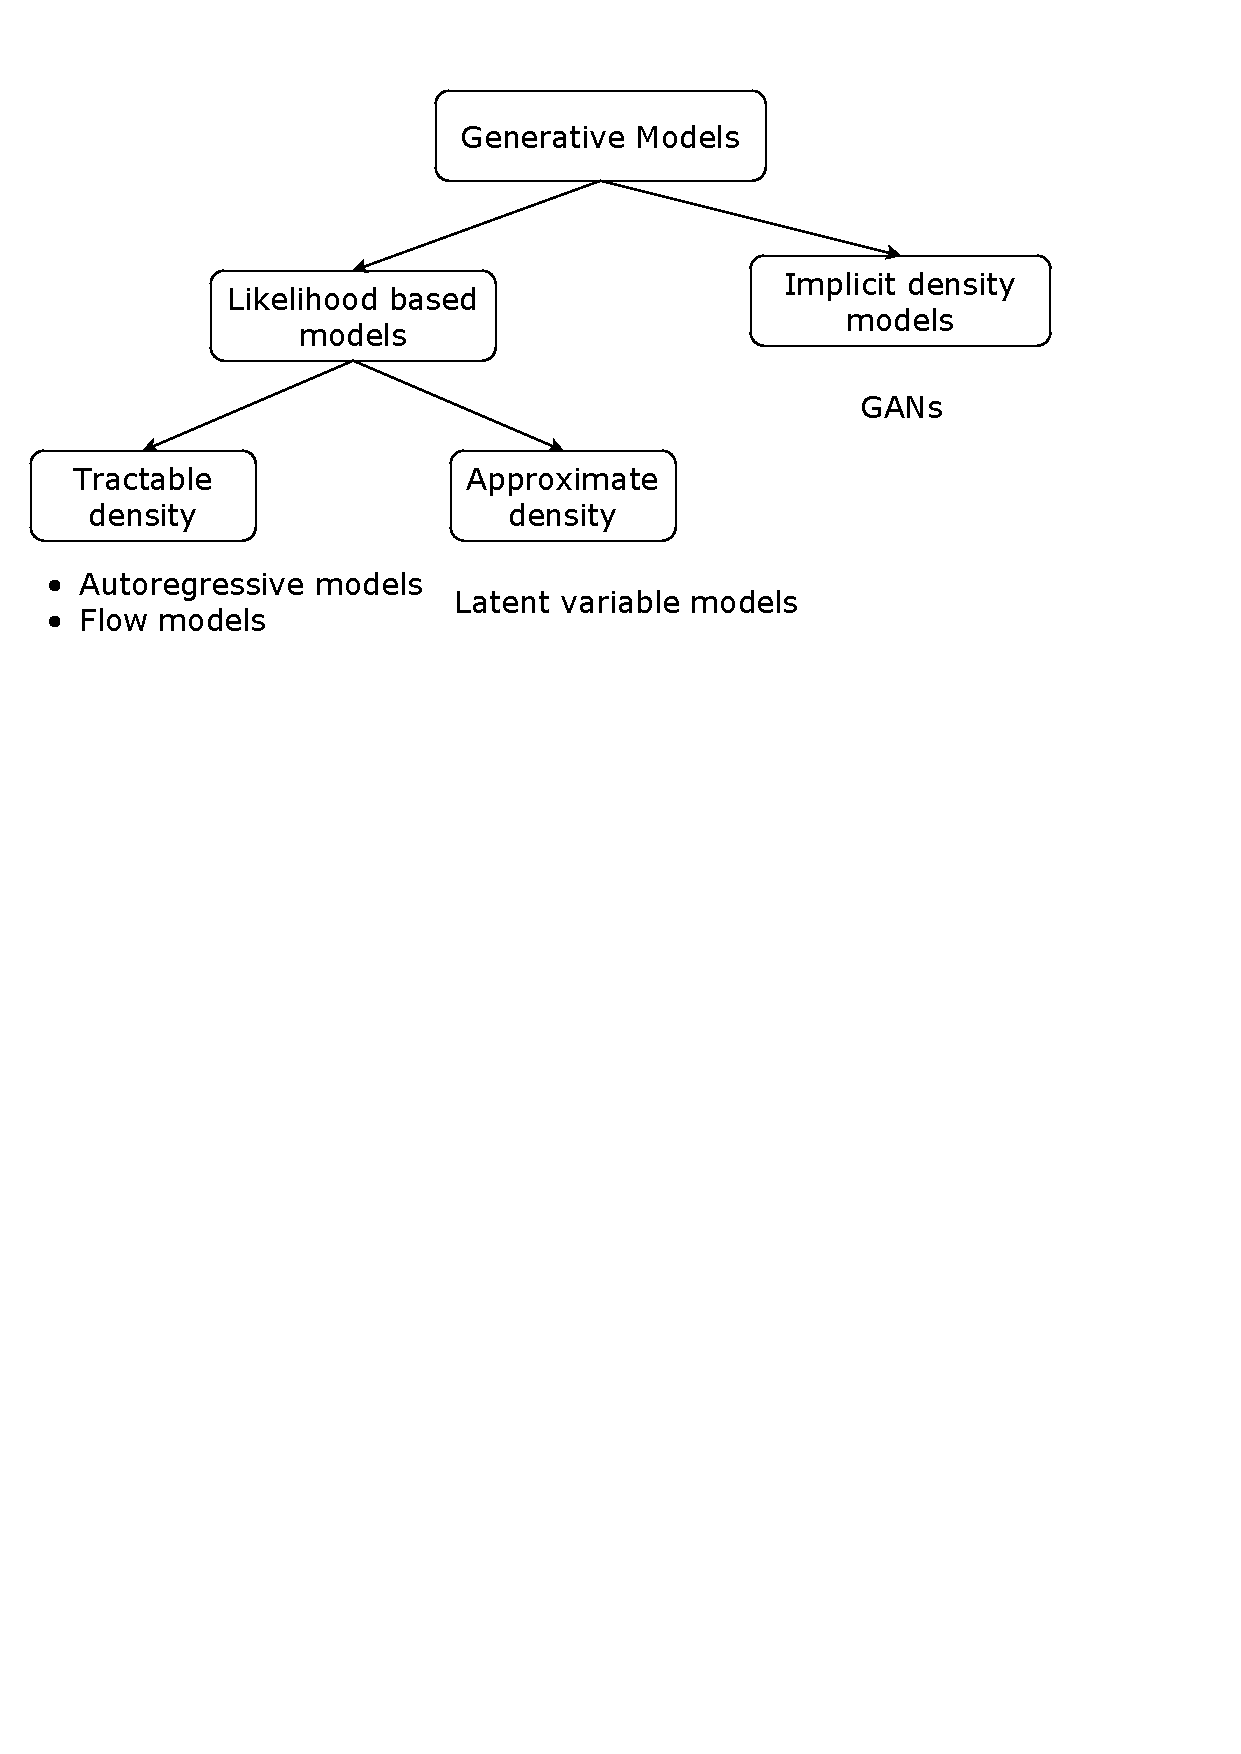
\includegraphics[width=1.0\linewidth]{figs/generative_models_zoo.pdf}
        \label{fig:generative_models_zoo}
    \end{figure}
\end{frame}
\begin{frame}{Motivation}
    \begin{figure}
        \centering
        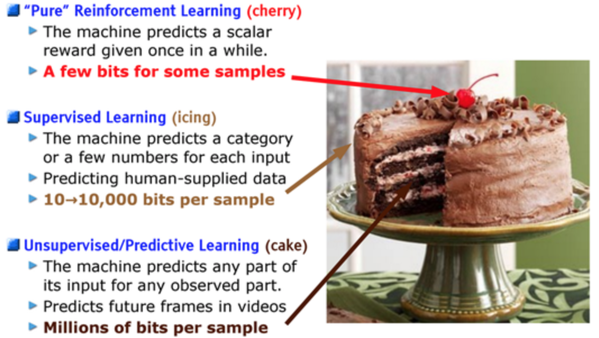
\includegraphics[width=\linewidth]{figs/unsupervised_cake.png}
        \label{fig:unsupervised_cake}
    \end{figure}
\vfill
\hrule\medskip
{\scriptsize LeCun, NIPS 2016 Keynote}
\end{frame}
%=======
\begin{frame}{Applications: Image generation (VAE)}
    \begin{figure}
        \centering
        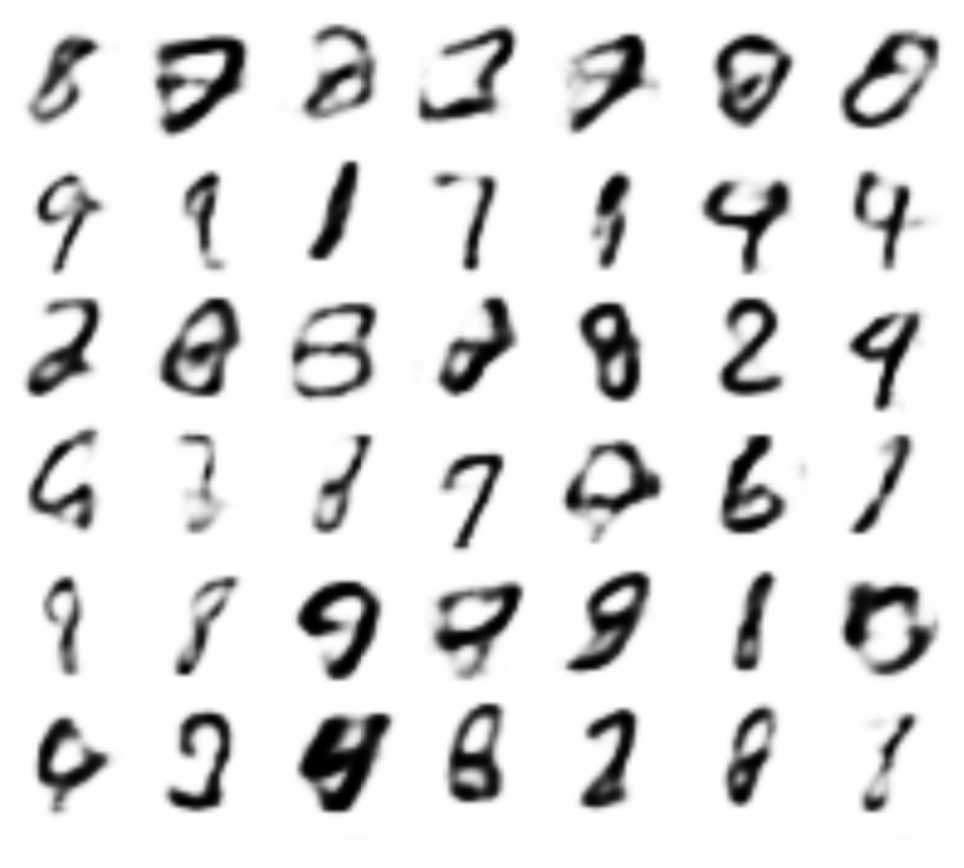
\includegraphics[width=0.5\linewidth]{figs/vae.png}
        \label{fig:vae}
    \end{figure}
\vfill
\hrule\medskip
{\scriptsize Kingma D. P., Welling M. Auto-encoding variational bayes \href{https://arxiv.org/pdf/1312.6114.pdf}{https://arxiv.org/pdf/1312.6114.pdf}}
\end{frame}
%=======
\begin{frame}{Applications: Image generation (DCGAN)}
    \begin{figure}
        \centering
        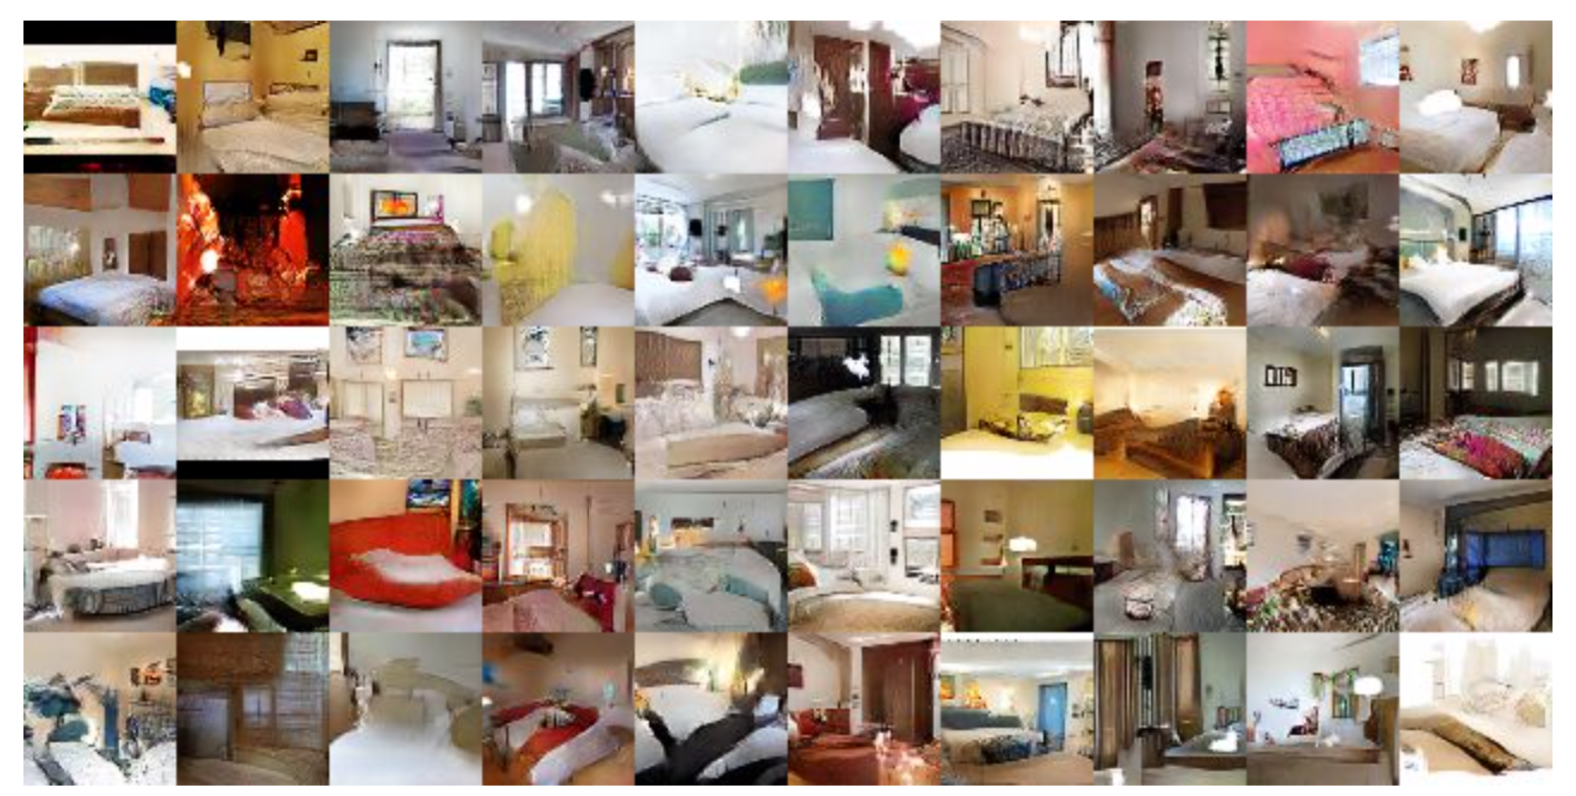
\includegraphics[width=1.0\linewidth]{figs/dcgan.png}
        \label{fig:dcgan}
    \end{figure}
\vfill
\hrule\medskip
{\scriptsize Radford A., Metz L., Chintala S. Unsupervised representation learning with deep convolutional generative adversarial networks  \href{https://arxiv.org/abs/1511.06434}{https://arxiv.org/abs/1511.06434}}
\end{frame}
%=======
\begin{frame}{Applications: SuperResolution (SRGAN)}
    \begin{figure}
        \centering
        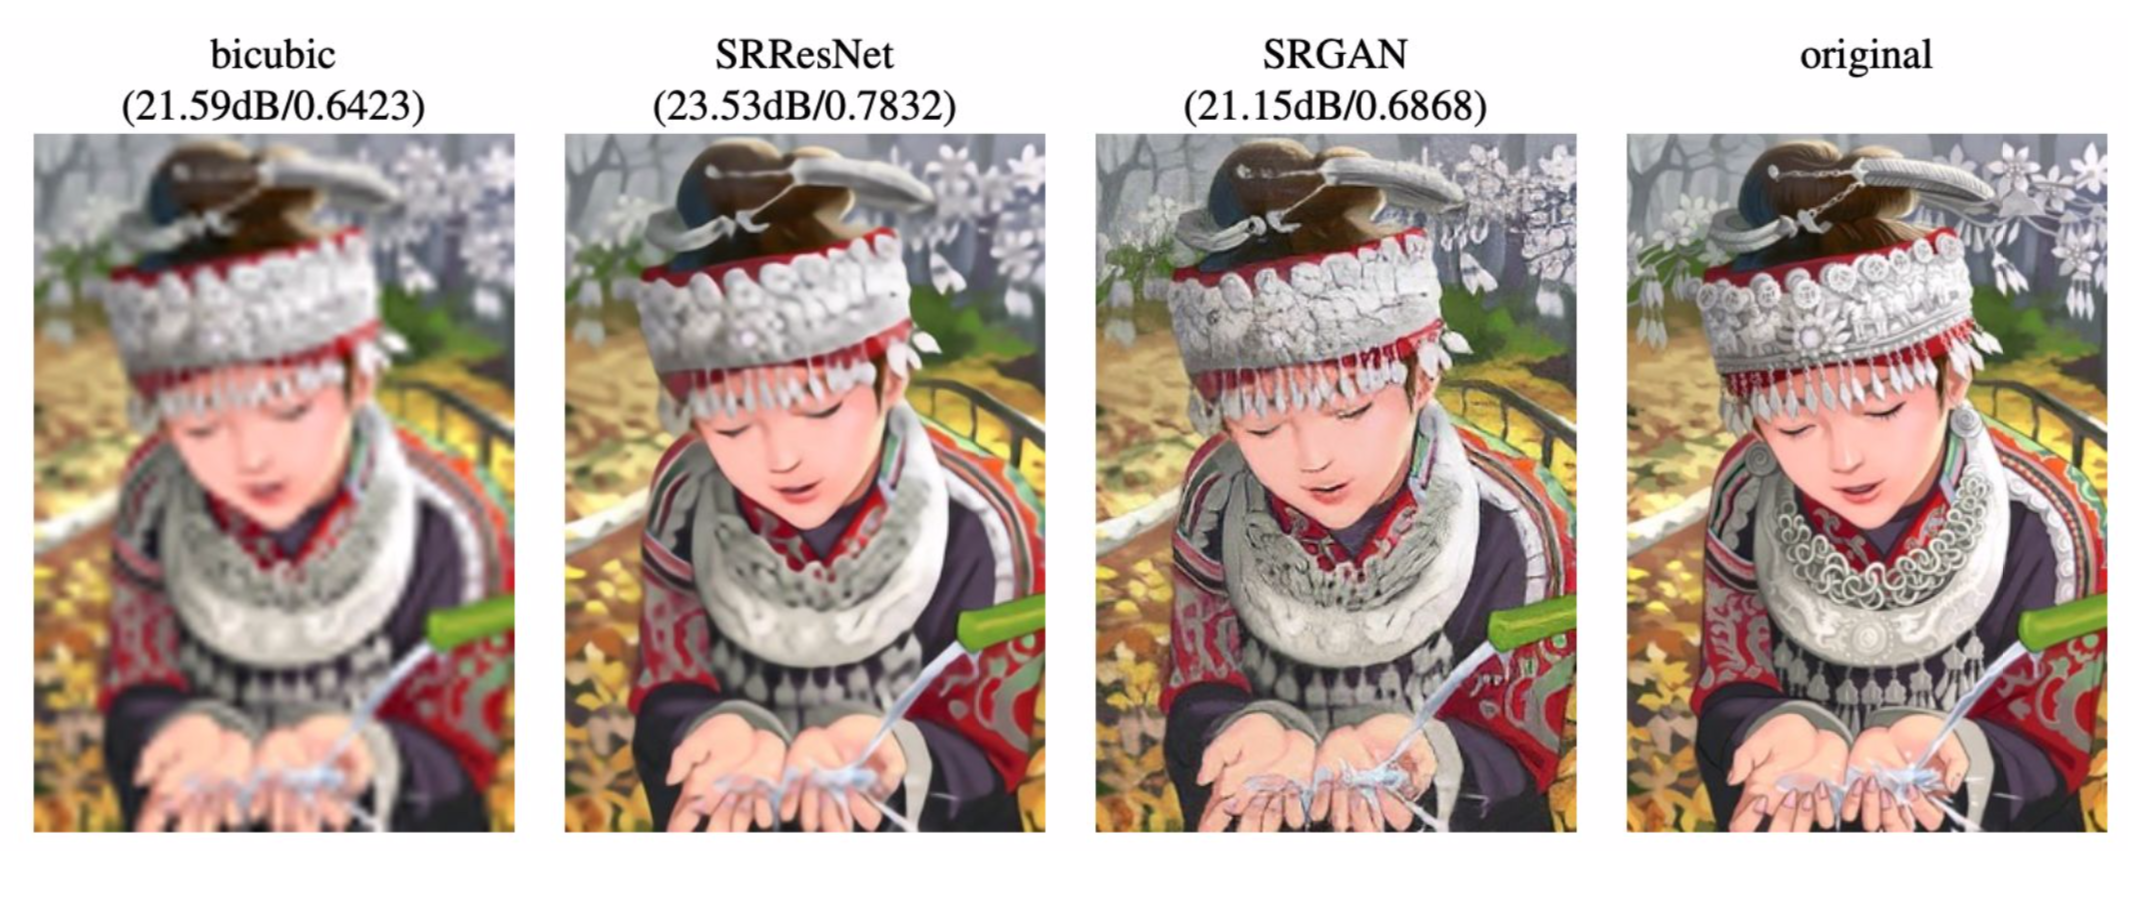
\includegraphics[width=1.0\linewidth]{figs/srgan.png}
        \label{fig:srgan}
    \end{figure}
\vfill
\hrule\medskip
{\scriptsize Ledig C. et al. Photo-realistic single image super-resolution using a generative adversarial network  \href{https://arxiv.org/abs/1609.04802}{https://arxiv.org/abs/1609.04802}}
\end{frame}
%=======
\begin{frame}{Applications: Domain translation (CycleGAN)}
    \begin{figure}
        \centering
        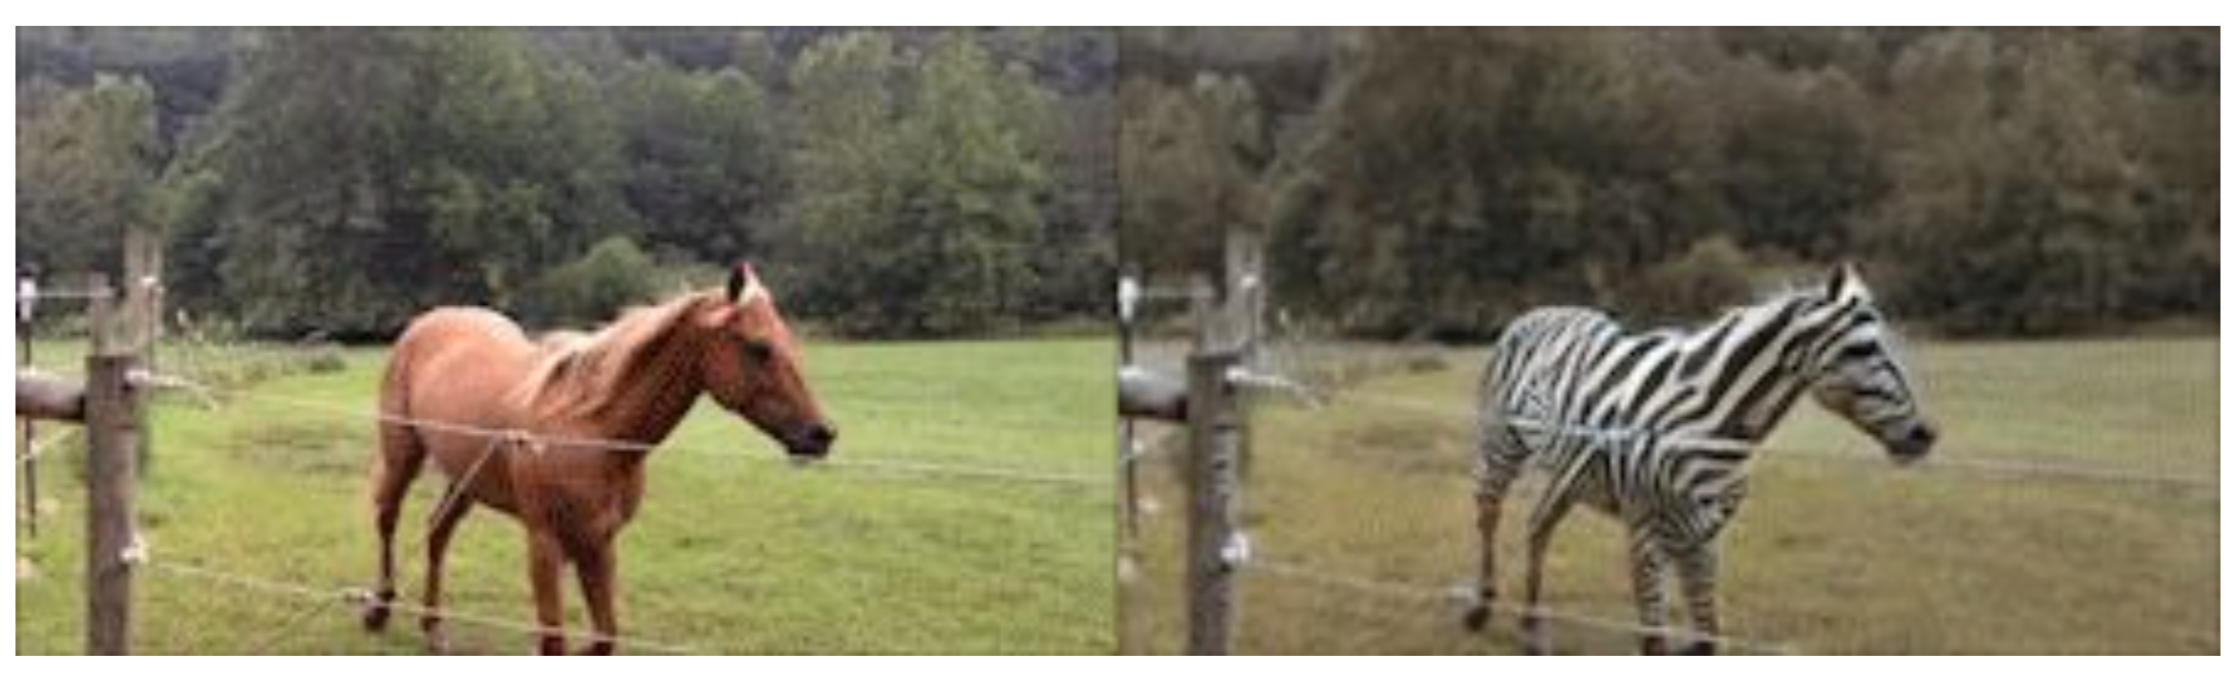
\includegraphics[width=1.0\linewidth]{figs/cyclegan.png}
        \label{fig:cyclegan}
    \end{figure}
\vfill
\hrule\medskip
{\scriptsize Zhu J. Y. et al. Unpaired image-to-image translation using cycle-consistent adversarial networks  \href{https://arxiv.org/abs/1703.10593}{https://arxiv.org/abs/1703.10593}}
\end{frame}
%=======
\begin{frame}{Applications: Face generation (StyleGAN)}
    \begin{figure}
        \centering
        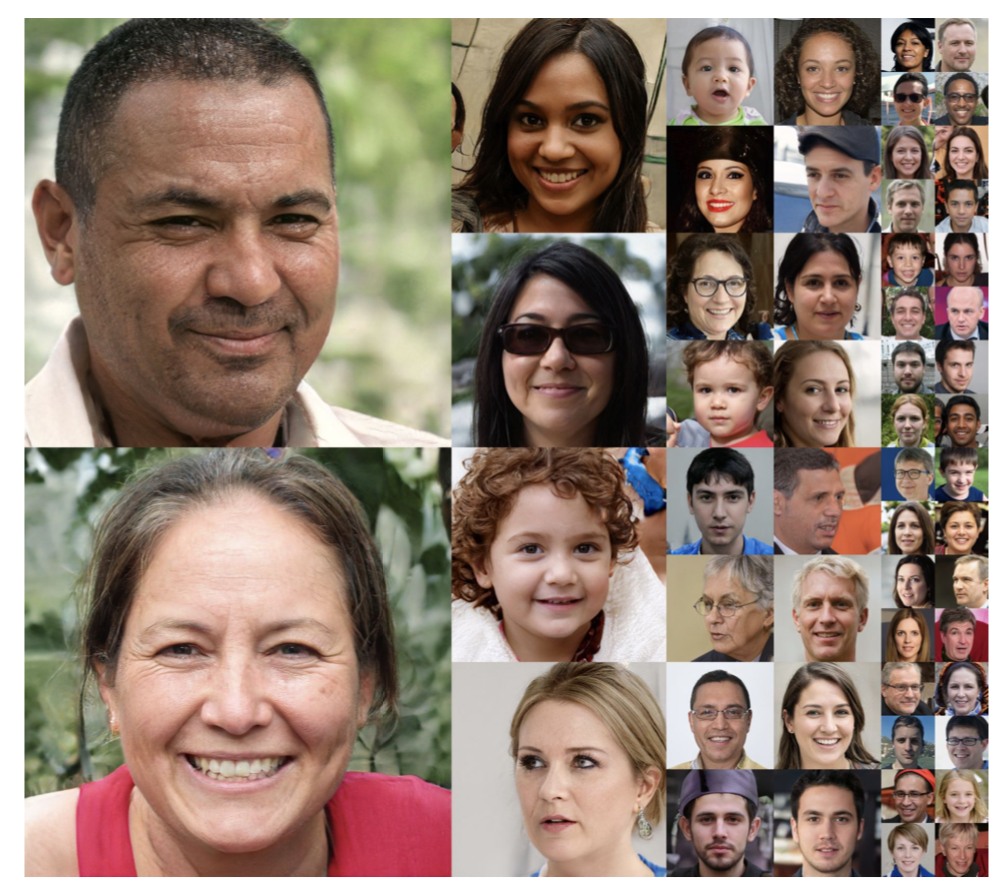
\includegraphics[width=0.65\linewidth]{figs/stylegan.png}
        \label{fig:stylegan}
    \end{figure}
\vfill
\hrule\medskip
{\scriptsize Karras T., Laine S., Aila T. A style-based generator architecture for generative adversarial networks  \href{https://arxiv.org/abs/1812.04948}{https://arxiv.org/abs/1812.04948}}
\end{frame}
%=======
\begin{frame}{Applications: Face generation (VQ-VAE-2)}
    \begin{figure}
        \centering
        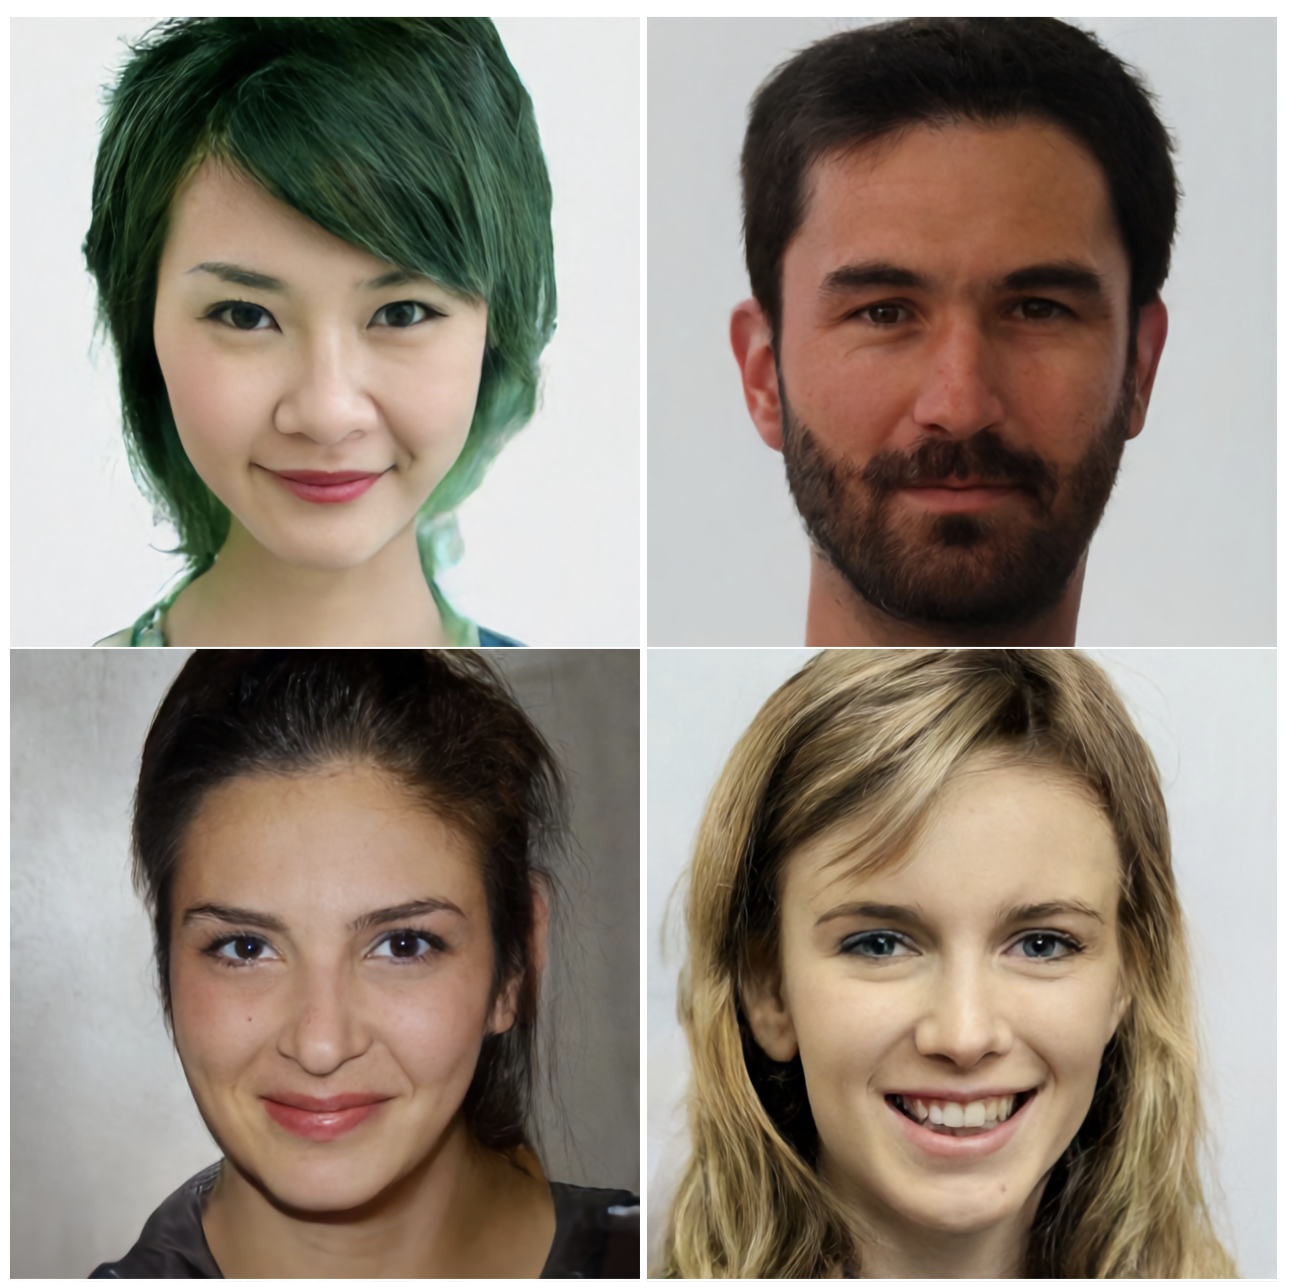
\includegraphics[width=0.65\linewidth]{figs/vq_vae.png}
        \label{fig:vq_vae}
    \end{figure}
\vfill
\hrule\medskip
{\scriptsize Razavi A., Oord A., Vinyals O. Generating Diverse High-Fidelity Images with VQ-VAE-2 \href{https://arxiv.org/abs/1906.00446}{https://arxiv.org/abs/1906.00446}}
\end{frame}
%=======
\begin{frame}{Applications}
\begin{itemize}
    \item Audio Generation (WaveNet, ...)
    \item Video Generation (DVD-GAN)
    \item NLP (Transformer, BERT, GPT-3, ...)
    \item Compression
\end{itemize}
\end{frame}
%--------------------------------------------------------------------------------
\section{Likelihood based models}
\begin{frame}{Problem Statement}
Given samples $\{\bx_i\}_{i=1}^n \in X$ from unknown distribution $\pi(\bx)$.

\begin{block}{Goal}
	learn a distribution $\pi(\bx)$ for 
	\begin{itemize}
	    \item evaluating $\pi(\bx)$ for new samples;
	    \item sampling from $\pi(\bx)$.
	\end{itemize}
\end{block}
\begin{block}{Challenge}
	 Data is complex and high-dimensional (curse of dimensionality).
\end{block}
\end{frame}
%=======
\begin{frame}{Histogram as a generative model}

\begin{minipage}[t]{0.6\columnwidth}
    The histogram is totally defined by
	\[
	    p_k = p(x = k) = \frac{\sum_{i=1}^k [x_i = k]}{n}.
	\]
	\textbf{Problem:} curse of dimensionality. \\
	\vspace{0.05cm} \\
	MNIST: 28x28 gray-scaled images \\
	$2^{28\times28} - 1$ parameters to specify $p(\bx)$ 
	\end{minipage}%
	\begin{minipage}[t]{0.4\columnwidth}
    \begin{figure}[h]
        \centering
        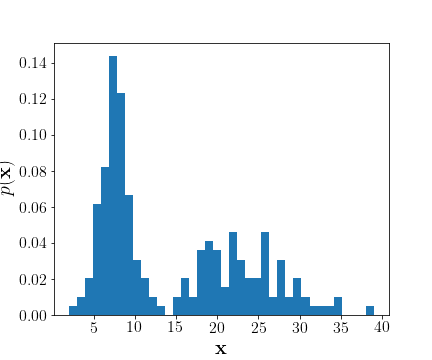
\includegraphics[width=\linewidth]{figs/histogram.png}
    \end{figure}
\end{minipage}
\[
    p(\bx) = p(x_1) \cdot p(x_2 | x_1) \cdot \dots \cdot p(x_m | x_{m-1}, \dots, x_1).
\]
\textbf{Question:} How many parameters do we need in these cases?
\[
    p(\bx) = p(x_1) \cdot p(x_2)\cdot \dots \cdot p(x_m).
\]
\[
    p(\bx) = p(x_1) \cdot p(x_2 | x_1) \cdot \dots \cdot p(x_m | x_{m-1}).
\]
\vspace{0.05cm}
\hrule\medskip
{\scriptsize  \href{https://sites.google.com/view/berkeley-cs294-158-sp20/home}{https://sites.google.com/view/berkeley-cs294-158-sp20/home}}
\end{frame}
%=======
\begin{frame}{Maximum likelihood}
    Fix probabilistic model $p(\bx | \btheta)$~-- the set of parameterized distributions . \\
    Instead of searching true $\pi(\bx)$ over all probability distributions, learn function approximation $p(\bx | \btheta) \approx \pi(\bx)$.
    
    \begin{block}{MLE problem}
    \vspace{-0.3cm}
    \[
        \btheta^* = \argmax_{\btheta} p(\bX | \btheta) = \argmax_{\btheta} \prod_{i=1}^n p(\bx_i | \btheta) = \argmax_{\btheta} \sum_{i=1}^n \log p(\bx_i | \btheta).
    \]
    \vspace{-0.1cm}
    \end{block}
    
    The problem is solved with SGD.
    \begin{block}{Requirements}
        \begin{itemize}
            \item efficiently compute $\log p(\bx | \btheta)$;
            \item efficiently compute gradient of $\log p(\bx | \btheta)$.
        \end{itemize}
    \end{block}
\end{frame}
\begin{frame}{Autoregressive model}
    \begin{block}{MLE problem}
    \vspace{-0.3cm}
    \[
        \btheta^* = \argmax_{\btheta} p(\bX | \btheta) = \argmax_{\btheta} \prod_{i=1}^n p(\bx_i | \btheta) = \argmax_{\btheta} \sum_{i=1}^n \log p(\bx_i | \btheta).
    \]
    \vspace{-0.1cm}
    \end{block}
    \begin{block}{Challenge}
    $p(\bx | \btheta)$ could be intractable.
    \end{block}
    \begin{block}{Likelihood as product of conditionals}
    Let $\bx = (x_1, \dots, x_m)$, $\bx_{1:i} = (x_1, \dots, x_i)$. Then 
    \[
        p(\bx | \btheta) = \prod_{i=1}^m p(x_i | \bx_{1:i - 1}, \btheta); \quad 
        \log p(\bx | \btheta) = \sum_{i=1}^m \log p(x_i | \bx_{1:i - 1}, \btheta).
    \]
    \end{block}
\end{frame}
%=======
\begin{frame}{Autoregressive models}
    \[
    \log p(\bx| \btheta) = \sum_{i=1}^m \log p(x_i | \bx_{1:i - 1}, \btheta)
    \]
    \begin{itemize}
        \item Each conditional could be modelled by neural network.
        \item To extend to high dimensions share parameters across conditionals.
        \item Sampling is sequential.
    \end{itemize}
    
\end{frame}
%=======
\begin{frame}{Char RNN (2015)}
	\begin{minipage}[t]{0.55\columnwidth}
		\begin{figure}[h]
			\centering
			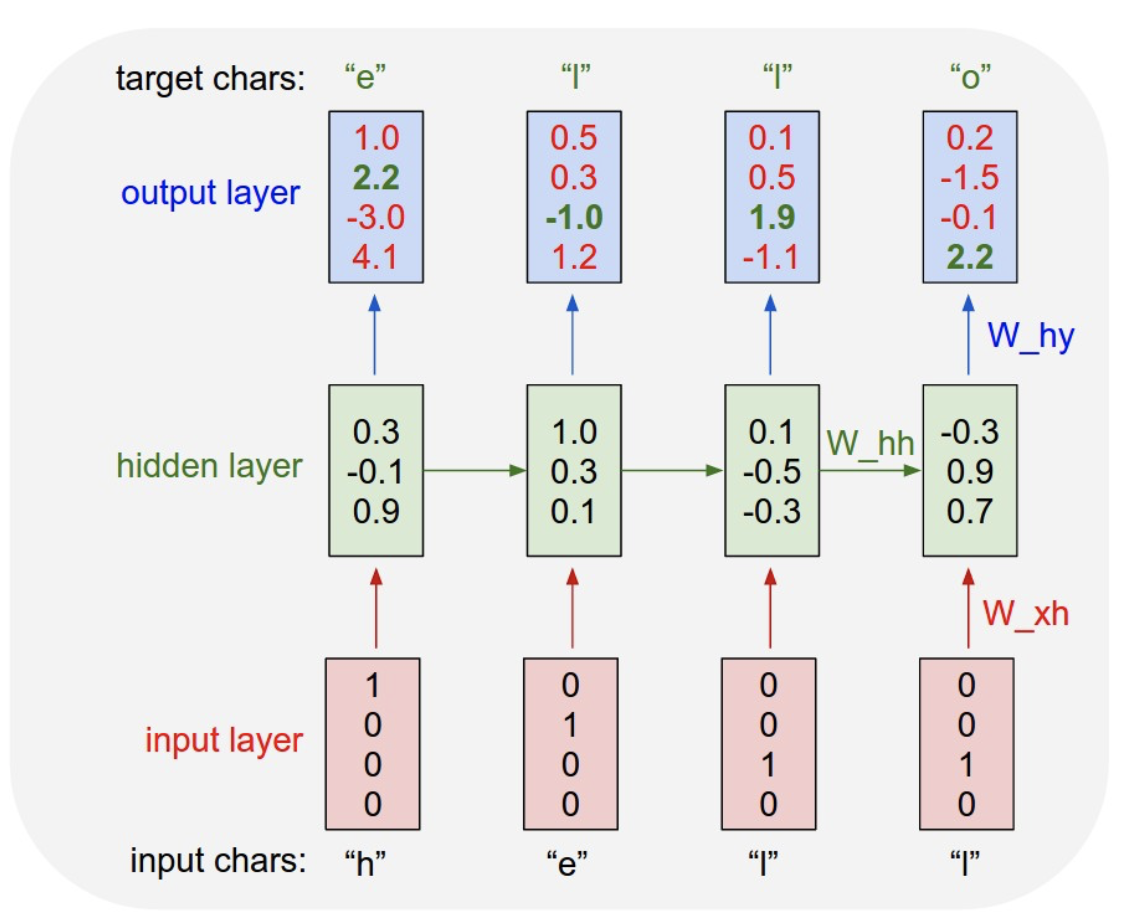
\includegraphics[width=1.0\linewidth]{figs/char_rnn.png}
		\end{figure}
	\end{minipage}%
	\begin{minipage}[t]{0.44\columnwidth}
		\begin{figure}[h]
			\centering
			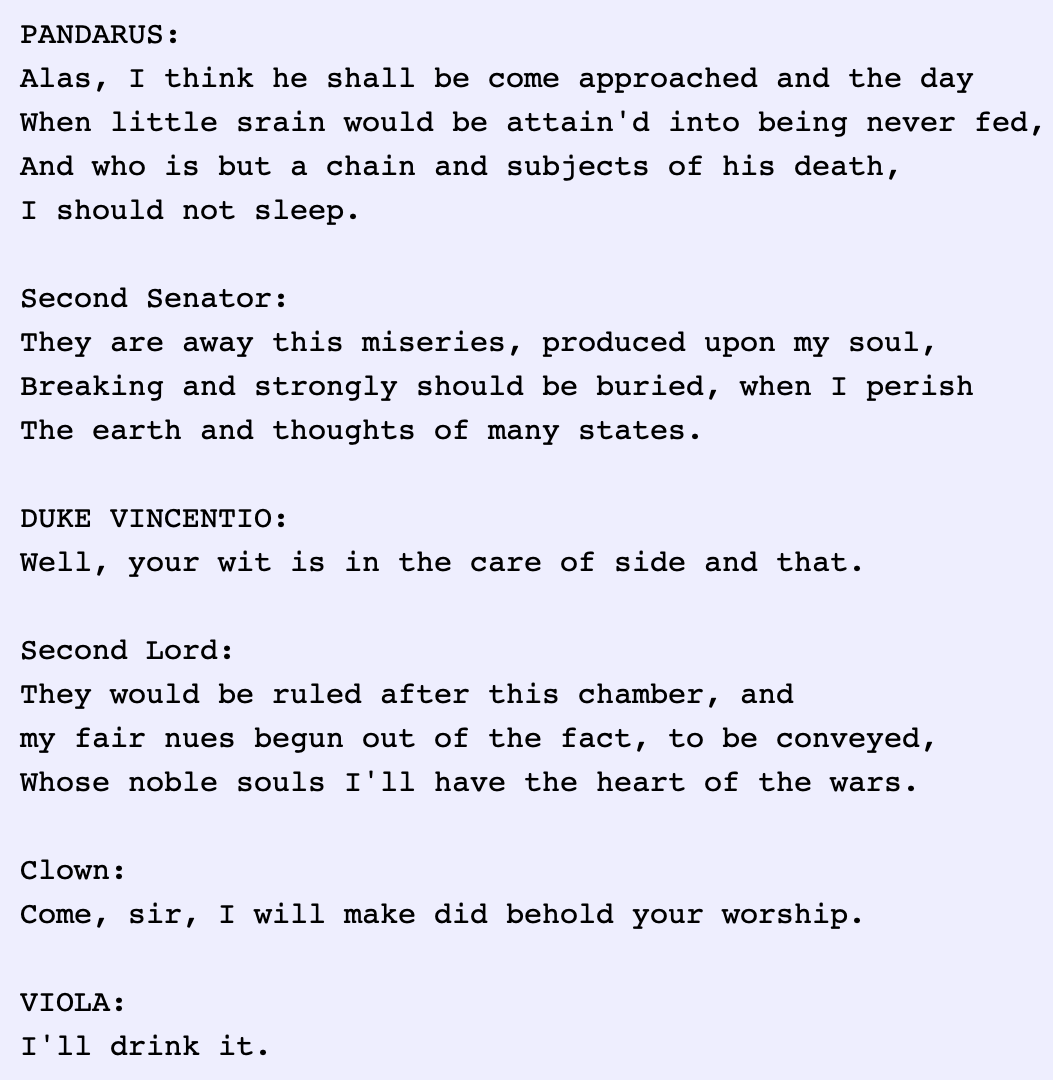
\includegraphics[width=1.0\linewidth]{figs/char_rnn_output.png}
		\end{figure}
	\end{minipage}
	\begin{block}{Drawback}
	Sequential computation of all conditionals $p(x_i | \bx_{1:i-1}, \btheta)$.
	\end{block}
\hrule\medskip
{\scriptsize  \href{http://karpathy.github.io/2015/05/21/rnn-effectiveness/}{http://karpathy.github.io/2015/05/21/rnn-effectiveness/}}
\end{frame}
%=======
\begin{frame}{MADE (2015)}
\begin{figure}
    \centering
    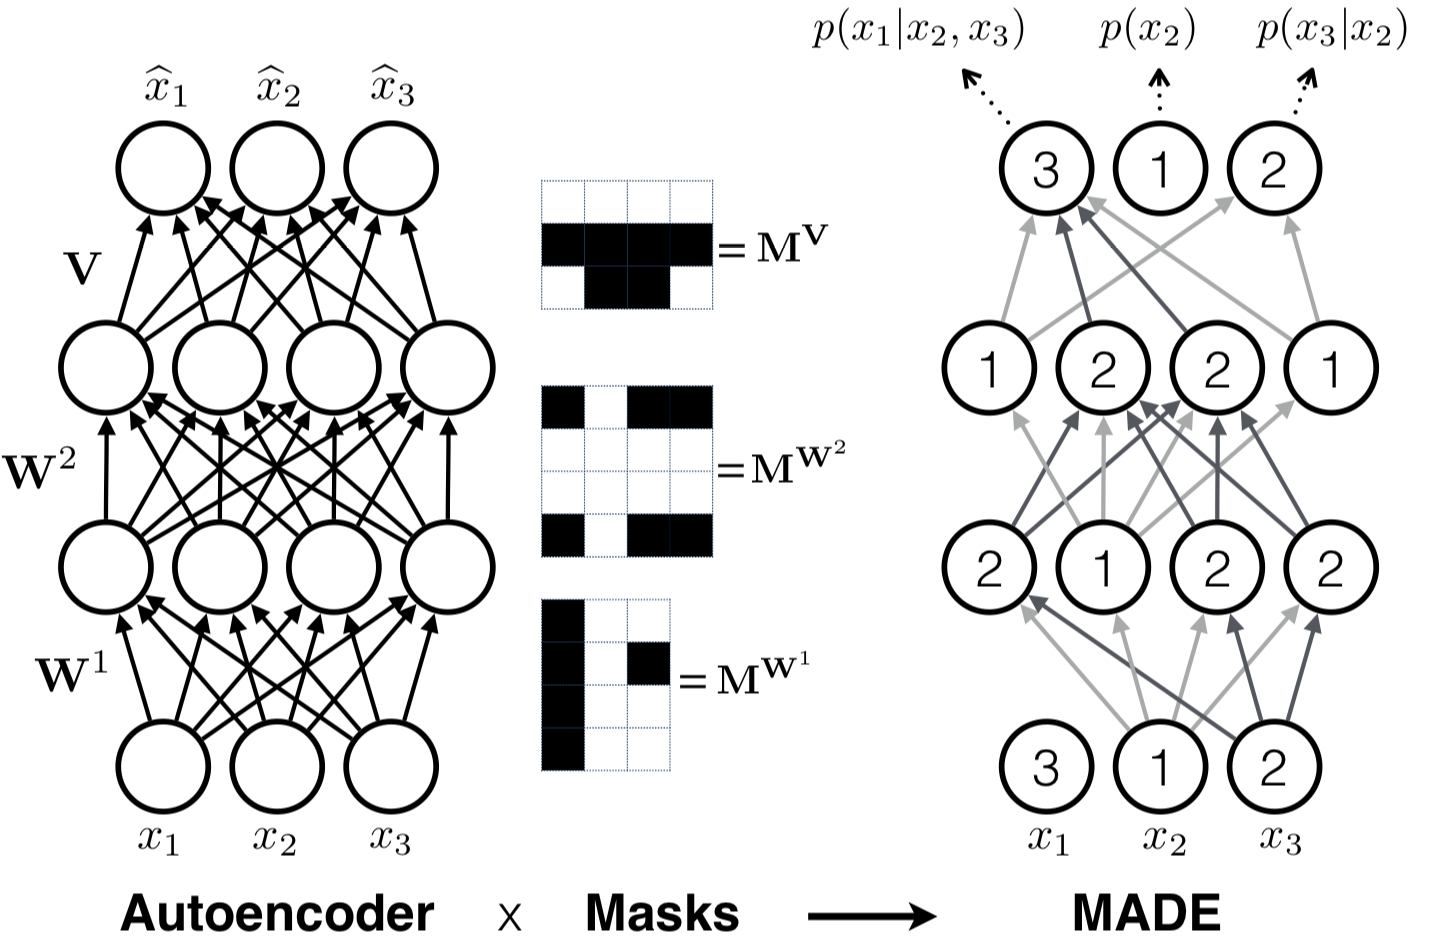
\includegraphics[width=0.9\linewidth]{figs/made.png}
    \label{fig:made}
\end{figure}
\vfill
\hrule\medskip
{\scriptsize Germain M. et al. Made: Masked autoencoder for distribution estimation \href{https://arxiv.org/pdf/1502.03509.pdf}{https://arxiv.org/pdf/1502.03509.pdf}}
\end{frame}
%=======
%=======
\begin{frame}{WaveNet (2016)}
\begin{block}{Goal}
Efficient generation of raw audio waveforms with natural sounds.
\end{block}
\begin{block}{Solution}
Autoregressive model
\[
    p(\bx| \btheta) = \prod_{t=1}^T p(x_t|\bx_{1:t-1}, \btheta).
\]
\end{block}
The model uses causal dilated convolutions.
\begin{figure}
    \centering
    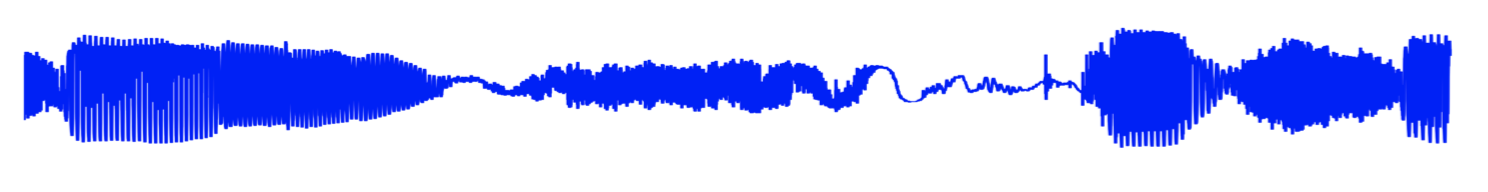
\includegraphics[width=0.9\linewidth]{figs/wavenet_ex.png}
\end{figure}
\vfill
\hrule\medskip
{\scriptsize Oord A. et al. Wavenet: A generative model for raw audio \href{https://arxiv.org/pdf/1609.03499.pdf}{https://arxiv.org/pdf/1609.03499.pdf}}
\end{frame}
%=======
\begin{frame}{WaveNet (2016)}
\begin{figure}
    \centering
    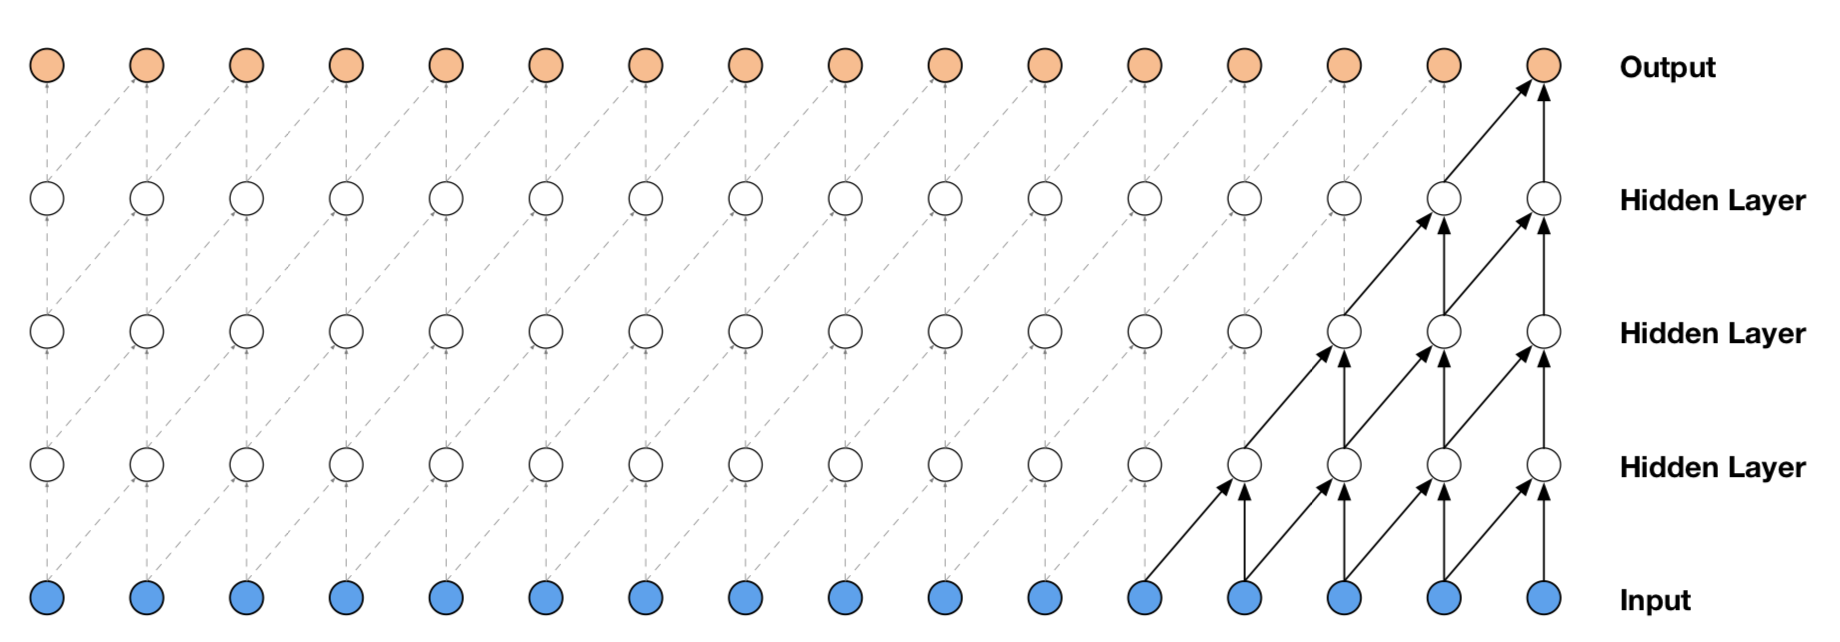
\includegraphics[width=0.9\linewidth]{figs/wavenet1.png}
\end{figure}

\begin{figure}
    \centering
    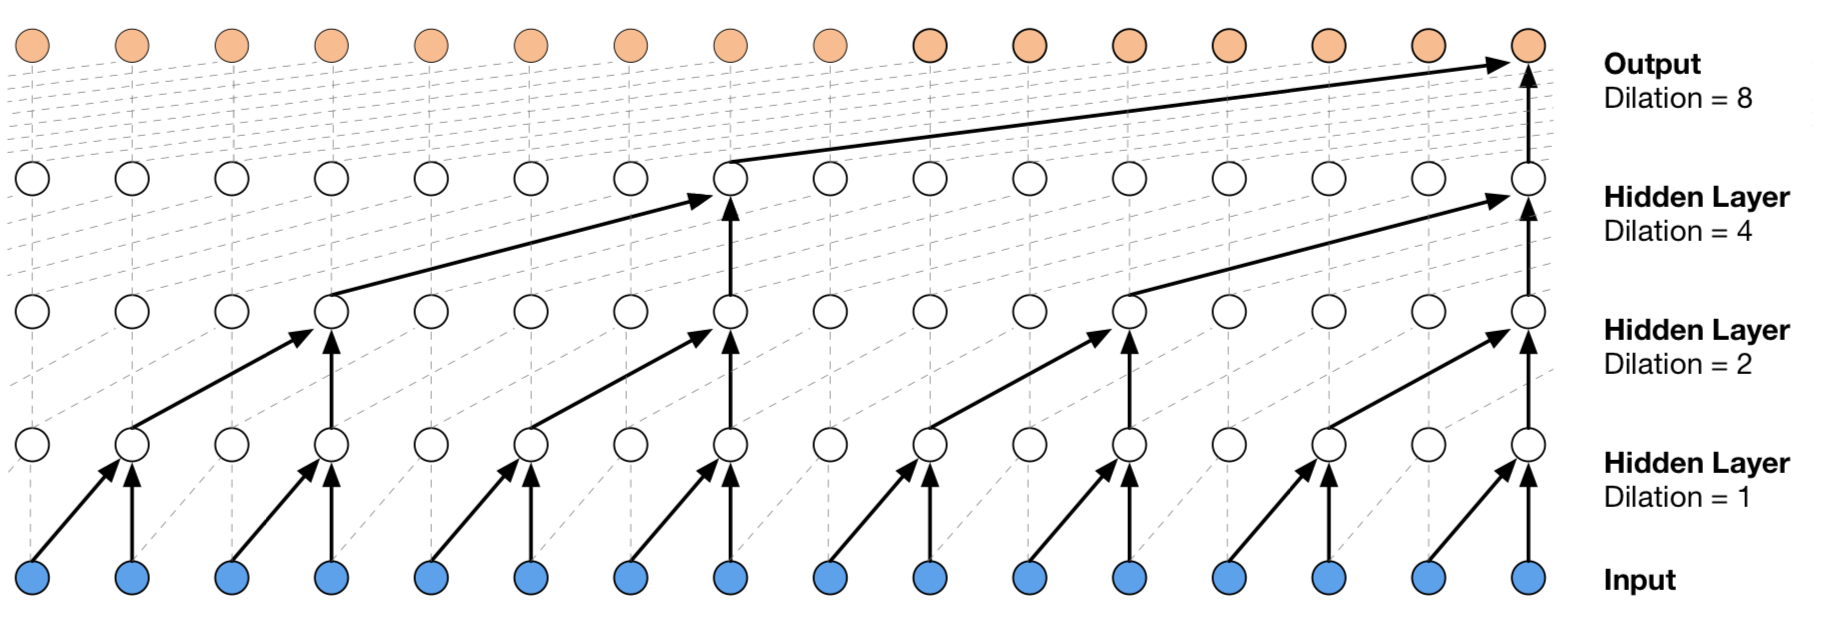
\includegraphics[width=0.9\linewidth]{figs/wavenet2.png}
\end{figure}
\vfill
\hrule\medskip
{\scriptsize Oord A. et al. Wavenet: A generative model for raw audio \href{https://arxiv.org/pdf/1609.03499.pdf}{https://arxiv.org/pdf/1609.03499.pdf}}
\end{frame}

%=======
\begin{frame}{PixelCNN (2016)}
\begin{block}{Goal}
Modeling the distribution of natural images.
\end{block}
\begin{block}{Solution}
Autoregressive model
\[
    p(\bx | \btheta) = \prod_{i=1}^{n^2} p(x_i|\bx_{1:i-1}, \btheta).
\]
\begin{itemize}
    \item masked convolutions;
    \item dependencies over RGB channels.
\end{itemize}
\end{block}
\vfill
\hrule\medskip
{\scriptsize Oord A., Kalchbrenner N., Kavukcuoglu K. Pixel recurrent neural networks \href{https://arxiv.org/pdf/1601.06759.pdf}{https://arxiv.org/pdf/1601.06759.pdf}}
\end{frame}
%=======
\begin{frame}{PixelCNN (2016)}
\begin{minipage}[t]{0.5\columnwidth}
	\begin{figure}[h]
		\centering
        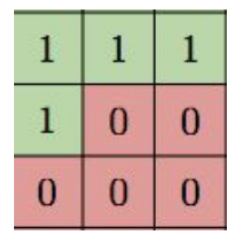
\includegraphics[width=0.35\linewidth]{figs/pixelcnn_0_1.png}
	\end{figure}
	\vspace{-0.1cm}
	\begin{figure}[h]
		\centering
        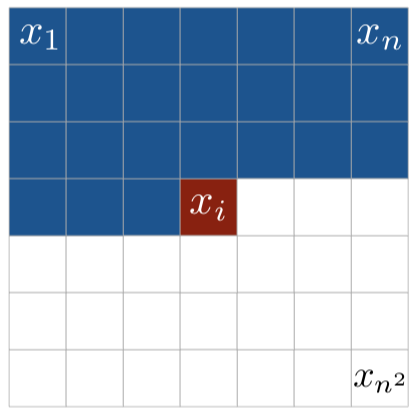
\includegraphics[width=0.7\linewidth]{figs/pixelcnn1.png}
	\end{figure}
	\end{minipage}%
	\begin{minipage}[t]{0.5\columnwidth}
	\begin{figure}[h]
		\centering
        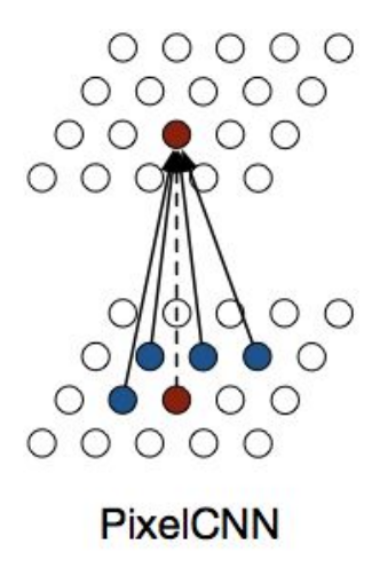
\includegraphics[width=0.5\linewidth]{figs/pixelcnn_0_2.png}
	\end{figure}
	\vspace{-0.4cm}
	\begin{figure}
		\centering
        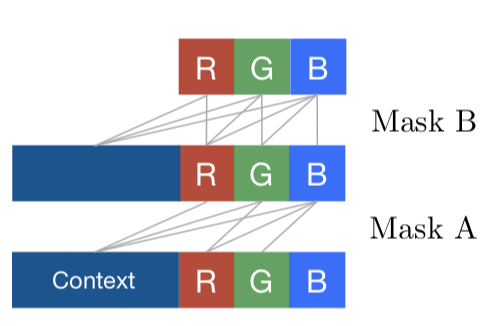
\includegraphics[width=0.65\linewidth]{figs/pixelcnn2.png}
	\end{figure}
\end{minipage}
\vfill
\hrule\medskip
{\scriptsize Oord A., Kalchbrenner N., Kavukcuoglu K. Pixel recurrent neural networks \href{https://arxiv.org/pdf/1601.06759.pdf}{https://arxiv.org/pdf/1601.06759.pdf}}
\end{frame}
%=======
\begin{frame}{Summary}
    \begin{itemize}
        \item Sampling from autoregressive models are trivial, but sequential
        \begin{itemize}
            \item sample $x_0 \sim p(x_0)$;
            \item sample $x_1 \sim p(x_1 | x_0)$;
            \item \dots.
        \end{itemize}
        \item Estimating probability:
        \[
            p(\bx) = \prod_{i=1}^m p(x_i | \bx_{1:i - 1}).
        \]
        \item Work on both continuous and discrete data.
        \item There is no natural way to do unsupervised learning.
    \end{itemize}
\end{frame}
%=======
\begin{frame}{References}
{\tiny
\begin{itemize}
	\item \textbf{MADE}: \textit{Masked Autoencoder for Distribution Estimation} \\
	\href{https://arxiv.org/pdf/1502.03509.pdf}{https://arxiv.org/pdf/1502.03509.pdf} \\
	\textbf{Summary}: Create masked autoencoder that models autoregression (autoregression allows to make the distribution properly normalized). Sampling is performed iteratively (to generate MNIST image 784 forward passes are needed). Discrete data.
	
	\item \textbf{PixelRNN + PixelCNN}: \textit{Pixel recurrent neural networks} \\
	\href{https://arxiv.org/abs/1601.06759}{https://arxiv.org/abs/1601.06759} \\
	\textbf{Summary}: 2 models are proposed: PixelRNN, PixelCNN. The models are autoregression and sampling is sequential. For RNN two types of LSTM blocks are used: Row LSTM and DiagonalBiLSTM. CNN uses Masked convolutions. RNN outperforms, but is slower.
	
	\item \textbf{GatedPixelCNN}: \textit{Conditional Image Generation with PixelCNN Decoders} \\
	\href{https://arxiv.org/pdf/1606.05328.pdf}{https://arxiv.org/pdf/1606.05328.pdf} \\
	\textbf{Summary}: Improvements for PixelCNN: gated units (like in lstm), horizontal+vertical stacks (remove blind spots). The result is now similar to PixelRNN.
	
	\item \textbf{WaveNet}: \textit{a Generative Model for Raw Audio} \\
	\href{https://arxiv.org/pdf/1609.03499.pdf}{https://arxiv.org/pdf/1609.03499.pdf} \\
	\textbf{Summary}: Model for autoregressive audio generation, inspired by PixelCNN. Use causal convolutions for the right conditioning, and dilated atrous convolution to extend receptive field.
	
	\item \textbf{PixelCNN++}: \textit{Improving the PixelCNN with Discretized Logistic Mixture Likelihood and Other Modifications} \\
	\href{https://arxiv.org/pdf/1701.05517.pdf}{https://arxiv.org/pdf/1701.05517.pdf} \\
	\textbf{Summary}: Improved version of PixelCNN. Models mixture of logistic mixture distribution instead of softmax. Architectural modifications: skip connections, up/down sampling, dropout. Experiment with dequantization: discretization works better.
	
	\item \textbf{PixelSNAIL}: \textit{An Improved Autoregressive Generative Model} \\
	\href{https://arxiv.org/pdf/1712.09763.pdf}{https://arxiv.org/pdf/1712.09763.pdf} \\
	\textbf{Summary}: Autoregressive model. Uses masked causal convolutions. Adjust self-attention to PixelCNN.
\end{itemize}
}
\end{frame}

\end{document} 